\documentclass[border=6pt]{standalone}
\usepackage{amsmath,amssymb}
\usepackage{tikz}
\usetikzlibrary{decorations.pathreplacing,calc,positioning}
% TikZ styles and helpers shared by figures/circuits.tex and figures/circuits_qsvt.tex
\tikzset{
  wire/.style={line width=0.55pt},
  gate/.style={draw,fill=white,minimum height=6.2mm,minimum width=7.5mm,inner sep=1.5pt,font=\small,line width=0.55pt},
  wgate/.style={gate,minimum width=13mm},
  ctrl/.style={circle,fill=black,inner sep=0pt,minimum size=1.9mm},
  octrl/.style={circle,draw,fill=white,inner sep=0pt,minimum size=1.9mm,line width=0.55pt},
  targ/.style={circle,draw,inner sep=0pt,minimum size=3.2mm,line width=0.55pt},
  meter/.style={draw,fill=white,minimum height=6.2mm,minimum width=7.5mm,line width=0.55pt},
  reg/.style={font=\small,anchor=east},
  blk/.style={font=\footnotesize,anchor=north,text=black!65},
  st/.style={font=\footnotesize,anchor=south,text=blue!45!black},
  brace/.style={decorate,decoration={brace,mirror,amplitude=2.2pt},line width=0.4pt,black!60},
  slash/.style={},
}
\newcommand{\slashwire}[3]{% x y label : the /n mark on a multi-qubit wire
  \draw[line width=0.7pt] (#1cm-1.3mm,#2cm-1.6mm) -- (#1cm+1.3mm,#2cm+1.6mm);
  \node[font=\scriptsize,anchor=south west,inner sep=0.4pt] at (#1cm+0.9mm,#2cm+0.9mm) {#3};}
\newcommand{\vsep}[3]{% x ybot ytop : a dashed block boundary
  \draw[dashed,black!45,line width=0.4pt] (#1cm,#2cm) -- (#1cm,#3cm);}


% box spanning wires: x, ytop, ybot, width(cm), label
\newcommand{\mb}[5]{\draw[fill=white,line width=0.55pt] (#1-#4/2,#2+0.31) rectangle (#1+#4/2,#3-0.31); \node[font=\small] at (#1,{(#2+#3)/2}) {#5};}
\newcommand{\gt}[3]{\node[gate] at (#1,#2) {#3};}
\newcommand{\wg}[4]{\node[gate,minimum width=#3] at (#1,#2) {#4};}
\newcommand{\ct}[2]{\node[ctrl] at (#1,#2) {};}
\newcommand{\oc}[2]{\node[octrl] at (#1,#2) {};}
\newcommand{\vl}[3]{\draw[wire] (#1,#2) -- (#1,#3);}
\newcommand{\tg}[2]{\node[targ] at (#1,#2) {}; \draw[wire] (#1,#2-0.16) -- (#1,#2+0.16);}
\newcommand{\meas}[2]{\node[meter] at (#1,#2) {}; \draw[wire] (#1-0.25,#2-0.12) arc (160:20:0.27); \draw[wire,-latex] (#1,#2-0.12) -- (#1+0.2,#2+0.12);}
\newcommand{\wires}[3]{\foreach \y in {#3} {\draw[wire] (#1,\y) -- (#2,\y);}}
\newcommand{\lab}[3]{\node[reg] at (#1,#2) {#3};}
\definecolor{hitp}{RGB}{118,68,160}
\definecolor{classic}{RGB}{90,90,90}
\newcommand{\cbox}[6]{\draw[rounded corners=3pt,fill=black!4,draw=black!45,line width=0.5pt] (#1,#2) rectangle (#3,#4); \node[font=\footnotesize,align=center,text width=#6] at ({(#1+#3)/2},{(#2+#4)/2}) {#5};}
\begin{document}

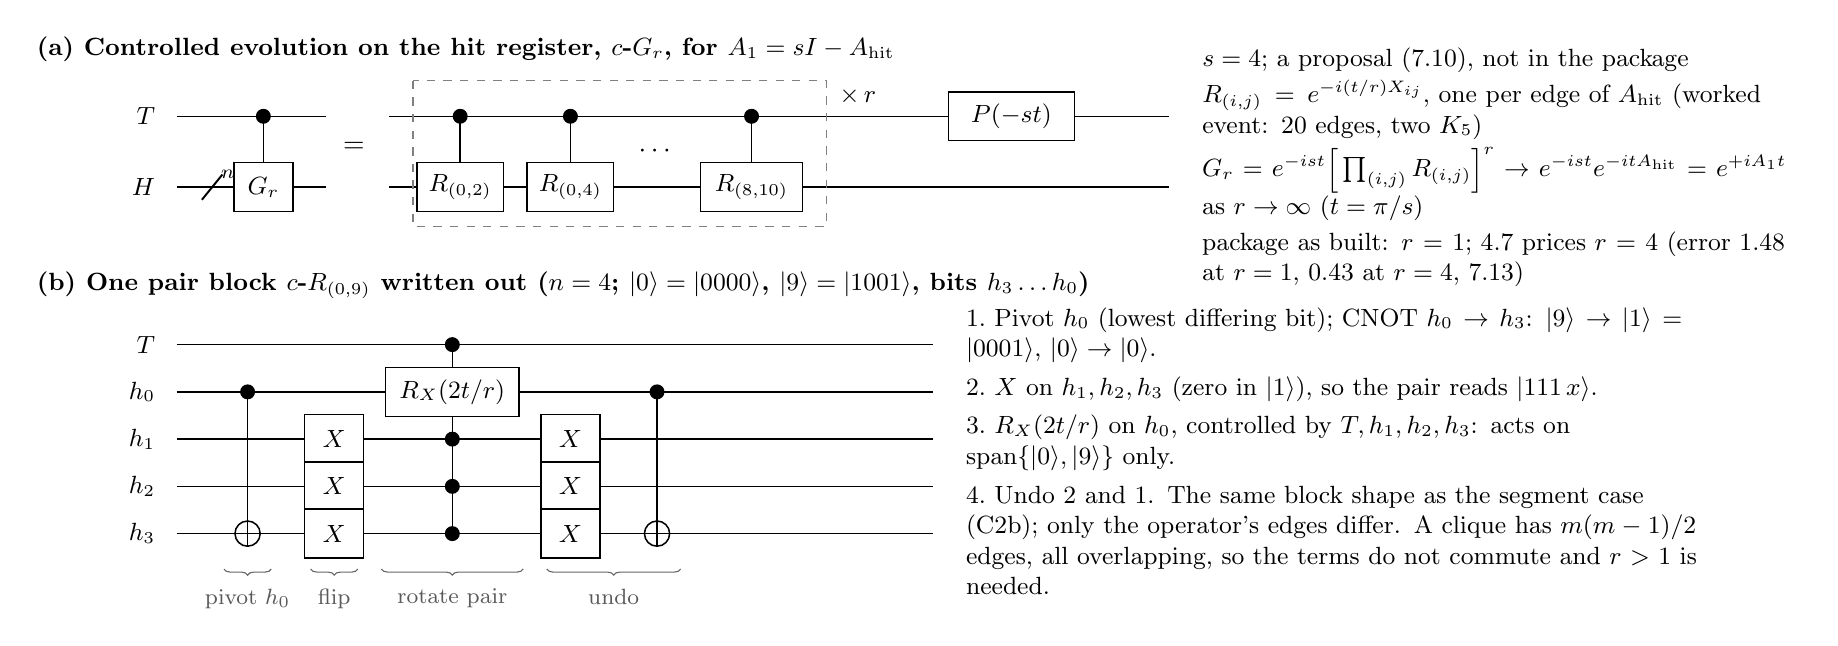
\begin{tikzpicture}[x=1cm,y=1cm]
% (a) hit operator controlled evolution with r product steps
\node[anchor=west,font=\small\bfseries] at (-1.9,1.25) {(a) Controlled evolution on the hit register, $c\text{-}G_r$, for $A_1=sI-A_{\rm hit}$};
\lab{-0.15}{0.4}{$T$} \lab{-0.15}{-0.5}{$H$}
\wires{0}{1.9}{0.4,-0.5} \slashwire{0.45}{-0.5}{$n$}
\ct{1.1}{0.4} \vl{1.1}{0.4}{-0.5} \gt{1.1}{-0.5}{$G_r$}
\node at (2.25,0) {$=$};
\wires{2.7}{12.6}{0.4,-0.5}
\draw[dashed,black!50] (3.0,0.85) rectangle (8.25,-1.0);
\ct{3.6}{0.4} \vl{3.6}{0.4}{-0.5} \wg{3.6}{-0.5}{11mm}{$R_{(0,2)}$}
\ct{5.0}{0.4} \vl{5.0}{0.4}{-0.5} \wg{5.0}{-0.5}{11mm}{$R_{(0,4)}$}
\node at (6.1,-0.05) {$\cdots$};
\ct{7.3}{0.4} \vl{7.3}{0.4}{-0.5} \wg{7.3}{-0.5}{13mm}{$R_{(8,10)}$}
\node[font=\small] at (8.65,0.65) {$\times\,r$};
\wg{10.6}{0.4}{16mm}{$P(-st)$}
\node[font=\small,anchor=west,text width=7.6cm] at (12.9,-0.25) {$s=4$; a proposal (7.10), not in the package\\[2pt] $R_{(i,j)}=e^{-i(t/r)X_{ij}}$, one per edge of $A_{\rm hit}$ (worked event: 20 edges, two $K_5$)\\[2pt] $G_r=e^{-ist}\Big[\prod_{(i,j)}R_{(i,j)}\Big]^{r}\to e^{-ist}e^{-itA_{\rm hit}}=e^{+iA_1t}$ as $r\to\infty$ ($t=\pi/s$)\\[2pt] package as built: $r=1$; 4.7 prices $r=4$ (error 1.48 at $r=1$, 0.43 at $r=4$, 7.13)};
% (b) pair block (0,9) on n=4
\begin{scope}[shift={(0,-3.1)}]
\node[anchor=west,font=\small\bfseries] at (-1.9,1.35) {(b) One pair block $c\text{-}R_{(0,9)}$ written out ($n=4$; $|0\rangle=|0000\rangle$, $|9\rangle=|1001\rangle$, bits $h_3\ldots h_0$)};
\lab{-0.15}{0.6}{$T$}
\lab{-0.15}{0}{$h_0$} \lab{-0.15}{-0.6}{$h_1$} \lab{-0.15}{-1.2}{$h_2$} \lab{-0.15}{-1.8}{$h_3$}
\wires{0}{9.6}{0.6,0,-0.6,-1.2,-1.8}
\ct{0.9}{0} \vl{0.9}{0}{-1.8} \tg{0.9}{-1.8}
\gt{2.0}{-0.6}{$X$} \gt{2.0}{-1.2}{$X$} \gt{2.0}{-1.8}{$X$}
\ct{3.5}{0.6} \ct{3.5}{-0.6} \ct{3.5}{-1.2} \ct{3.5}{-1.8} \vl{3.5}{0.6}{-1.8}
\wg{3.5}{0}{17mm}{$R_X(2t/r)$}
\gt{5.0}{-0.6}{$X$} \gt{5.0}{-1.2}{$X$} \gt{5.0}{-1.8}{$X$}
\ct{6.1}{0} \vl{6.1}{0}{-1.8} \tg{6.1}{-1.8}
\draw[brace] (0.6,-2.25) -- (1.2,-2.25); \node[blk] at (0.9,-2.38) {pivot $h_0$};
\draw[brace] (1.7,-2.25) -- (2.3,-2.25); \node[blk] at (2.0,-2.38) {flip};
\draw[brace] (2.6,-2.25) -- (4.4,-2.25); \node[blk] at (3.5,-2.38) {rotate pair};
\draw[brace] (4.7,-2.25) -- (6.4,-2.25); \node[blk] at (5.55,-2.38) {undo};
\node[font=\small,anchor=west,text width=9.4cm] at (9.9,-0.75) {1.\ Pivot $h_0$ (lowest differing bit); CNOT $h_0\to h_3$: $|9\rangle\to|1\rangle=|0001\rangle$, $|0\rangle\to|0\rangle$.\\[3pt]
2.\ $X$ on $h_1,h_2,h_3$ (zero in $|1\rangle$), so the pair reads $|111\,x\rangle$.\\[3pt]
3.\ $R_X(2t/r)$ on $h_0$, controlled by $T,h_1,h_2,h_3$: acts on $\mathrm{span}\{|0\rangle,|9\rangle\}$ only.\\[3pt]
4.\ Undo 2 and 1. The same block shape as the segment case (C2b); only the operator's edges differ. A clique has $m(m-1)/2$ edges, all overlapping, so the terms do not commute and $r>1$ is needed.};
\end{scope}
\end{tikzpicture}
\end{document}
